% Build from this directory with latexmk -pdf extended_appendix.tex.
\documentclass{article}
\usepackage[T1]{fontenc}
\usepackage{iclr2027-style/iclr2027_conference,times}
\usepackage{amsmath,amssymb,amsthm,mathtools}
\usepackage{graphicx,booktabs,tabularx,array}
\usepackage{algorithm,algpseudocode}
\usepackage{xcolor}
\usepackage{xurl}
\usepackage[colorlinks=true,linkcolor=blue!55!black,citecolor=blue!55!black,urlcolor=blue!55!black]{hyperref}
\newcommand{\PaperTitleEN}{Feature Geometry for Data-Pool Screening: Utility, Stability, and Limits}
\newcommand{\PaperKeywordsEN}{data selection, data-pool screening, frozen representations, optimal experimental design, distribution shift, empirical evaluation}

\hypersetup{pdfauthor={Anonymous},pdfkeywords={\PaperKeywordsEN}}
\hypersetup{pdftitle={\PaperTitleEN}}
\newcommand{\R}{\mathbb{R}}
\newcommand{\E}{\mathbb{E}}
\newcommand{\tr}{\operatorname{tr}}
\newcommand{\reff}{r_{\mathrm{eff}}}
\newcommand{\cC}{\mathcal{C}}
\newcommand{\cQ}{\mathcal{Q}}
\newcommand{\norm}[1]{\left\lVert#1\right\rVert}
\newtheorem{proposition}{Proposition}
\newtheorem{lemma}{Lemma}
\graphicspath{{figures/}}
\brokenpenalty=10000
% Generated from recorded E2b outcome tables.
\newcommand{\MainRecall}{98.333}
\newcommand{\MainRegret}{0.001311}
\newcommand{\MainReduction}{50.110}
% Supplemental diagnostics: post-hoc 2026-09-16 run.
\newcommand{\BootstrapRecall}{97.42}
\newcommand{\BootstrapMMDRecall}{97.85}
\newcommand{\BootstrapOverlap}{85.15}
\newcommand{\BrierErrorOverlap}{29.17}
\newcommand{\BrierSquaredOverlap}{30.83}
\newcommand{\BrierNLLOverlap}{90.83}
% Exploratory projection/readout follow-up, 2026-09-17.
\newcommand{\WorstErrorRecall}{40}
\newcommand{\WorstErrorGap}{1.66}
\newcommand{\ReadoutRidgeA}{98.33}
\newcommand{\ReadoutRidgeMMD}{99.38}
\newcommand{\RidgeSpan}{0.248}
\newcommand{\RidgeSelectedRegret}{0.001006}
\newcommand{\ReadoutLogisticA}{98.33}
\newcommand{\ReadoutLogisticMMD}{98.96}
\newcommand{\LogisticSpan}{14.65}
\newcommand{\LogisticSelectedRegret}{0.103}
% Exploratory decision-budget reanalysis, 2026-09-22.
\newcommand{\BudgetAFifty}{0.864511}
\newcommand{\BudgetMMDFifty}{0.864365}
\newcommand{\BudgetFull}{0.864118}
\newcommand{\BudgetRandomPrimary}{0.866030}
\newcommand{\BudgetFailureFifty}{2.083333}
% Independent matched decision timing and additive image-cost profiles.
\newcommand{\CostRidgeAResidentRatio}{0.3607}
\newcommand{\CostRidgeAImagesRatio}{1.0988}
\newcommand{\CostRidgeMMDResidentRatio}{0.1420}
\newcommand{\CostRidgeMMDImagesRatio}{1.0898}
\newcommand{\CostLogisticAResidentRatio}{0.1048}
\newcommand{\CostLogisticAImagesRatio}{0.5628}
\newcommand{\CostLogisticMMDResidentRatio}{0.1007}
\newcommand{\CostLogisticMMDImagesRatio}{0.5605}

% Record the effective layout for verify_draft.py without changing the style.
\makeatletter
\AtBeginDocument{%
  \typeout{ICLR-FORMAT-FONT: \f@size; \the\baselineskip}%
  \typeout{ICLR-FORMAT-TEXT: \the\textwidth; \the\textheight}%
  \typeout{ICLR-FORMAT-PAGE: \the\paperwidth; \the\paperheight}%
  \typeout{ICLR-FORMAT-PAR: \the\parindent; \the\parskip}%
}
\makeatother

\hypersetup{pdftitle={Extended Appendix: Feature Geometry for Data-Pool Screening}}
\title{Extended Appendix\\Feature Geometry for Data-Pool Screening}
\author{Anonymous authors}
\begin{document}
\maketitle
These materials accompany the revised paper and collect the extended derivations, archived protocols, and additional experimental diagnostics. They use the figures, generated tables, and bibliography in this directory.

\section{Additional spectral results and sketch diagnostics}

Marginal spectra and principal angles alone need not determine this pooled statistic: the same strengths can be assigned differently to shared and unshared directions. The following counterexample and local formula identify the missing directional information.

\begin{proposition}[Directional assignment matters]
There exist row-normalized pairs $(A,B_1)$ and $(A,B_2)$ with identical marginal singular spectra and principal angles between their row spaces, but different effective ranks after concatenation.
\end{proposition}
\begin{proof}
Take $A$ with four rows $e_1^\top$ and one row $e_2^\top$. Let $B_1$ have four rows $e_1^\top$ and one $e_3^\top$, and let $B_2$ have one row $e_1^\top$ and four $e_3^\top$. All three nonzero singular spectra are $(2,1)$; both row-space pairs have principal angles $(0,\pi/2)$. Their merged Gram spectra are $(8,1,1)$ and $(5,4,1)$, giving effective ranks approximately $2.6260$ and $2.8495$. The shared direction receives different energy despite the identical marginal summaries.
\end{proof}

Let $u,v$ be unit directions with $u^\top v=c\in[0,1]$. In the orthonormal basis $u,z$, where $v=cu+\sqrt{1-c^2}z$, the operator $a^2uu^\top+b^2vv^\top$ is
\begin{equation}
 \begin{pmatrix}
 a^2+b^2c^2 & b^2c\sqrt{1-c^2}\\
 b^2c\sqrt{1-c^2} & b^2(1-c^2)
 \end{pmatrix}.
\end{equation}
Its trace is $a^2+b^2$ and determinant $a^2b^2(1-c^2)$, so its eigenvalues are
\begin{equation}
 \lambda_{\pm}=\frac{a^2+b^2\pm\sqrt{(a^2-b^2)^2+4a^2b^2c^2}}{2}.
 \label{eq:local}
\end{equation}
At $c=1$, the second branch is zero. These pairs give a full spectrum when the associated blocks are mutually orthogonal and invariant for both source Grams; unpaired directions contribute their own eigenvalues. This compatibility condition matters because principal vectors need not be singular vectors.

If $G\succeq\widetilde G\succeq0$, inverse order implies $(P_0^{-1}+\sigma^{-2}G)^{-1}\preceq(P_0^{-1}+\sigma^{-2}\widetilde G)^{-1}$. Taking a trace against a PSD target moment preserves this order. More generally, suppose the sum of omitted sketch tails satisfies $0\preceq G-\widetilde G\preceq\delta I$. Define $B=P_0^{-1}+\sigma^{-2}\widetilde G$. Then
\begin{equation}
 \tr\!\left(\widehat C_T(B+\sigma^{-2}\delta I)^{-1}\right)
 \leq f_A(G)\leq\tr(\widehat C_TB^{-1}).
 \label{eq:interval}
\end{equation}
One admissible $\delta$ is the sum of valid spectral-norm bounds on each PSD tail. A candidate's proxy ordering is certified when its upper bound is below every competing lower bound. Thus interval width, as well as coverage, determines whether a sketch can resolve the next choice. The archived sweep evaluates this type of proxy comparison with its documented byte accounting.

The four-encoder, ten-construction-seed spectral sweep uses six overlap settings and four budgets, with 960 configurations per sketch rank. At ranks $10,20,50$, relative exact merged-effective-rank gains over rank-only are respectively $2.09,3.81,4.94\%$ for the Gram sketch and $4.90,5.48,5.68\%$ for DPP. These gains are in the geometry objective, not classification accuracy. Its entropy-continuity bounds follow the type of bound in \citet{audenaert2007}; all 2,880 selected-prefix intervals cover, but none of 7,200 evaluated greedy steps is certified. The archived source is \path{results/two_stage_controlled_rank_sweep_corrected_v3/}. These observations do not imply that every low-rank sketch must fail.

The separate E5 study compares sketch payloads to packed symmetric float64 Grams, not inflated dense storage. Among full-grid strategies whose mean byte ratio is at most $25\%$, the best selected-set match to Full-Gram greedy is $15.42\%$, achieved by adaptive rank cap 2 with mean byte ratio $14.91\%$. Its pairwise certificate rate is $3.91\%$ and fully certified selection rate zero. Adaptive fallback reaches full selected-set agreement but costs approximately $160\%$ of packed-Gram bytes on average when previous transmissions are counted. This fails the joint decision-and-communication requirement. The reference is Full-Gram greedy, not the exhaustive global minimizer.

\section{Archived implementation and stability details}

The CUDA reconstruction retains the original sample identifiers, candidate membership, preprocessing, and hyperparameters. All twelve Brier top-ten sets agree with the original study. Per-example loss means reproduce the reconstructed aggregate audit within $1.78\times10^{-15}$. For each target domain, 2,000 paired bootstrap draws resample its 2,048 test examples, sharing weights across combinations, encoders, and four losses. Fitted models and validation choices stay fixed; combination identifiers resolve ties. These draws measure sensitivity to test-example sampling. The original Brier top ten overlaps with NLL by $\BrierNLLOverlap\%$, raw squared loss by $\BrierSquaredOverlap\%$, and classification error by $\BrierErrorOverlap\%$ on average.

The archive retains historical experiment IDs to identify results without confusing them with the paper's scientific questions. The following paths are relative to the anonymous code repository:
\begin{itemize}
\item Shared-model and shift studies (E1): \path{results/target_conditioned/e1_synthetic/expanded_v3_controlled_rng/}.
\item PACS/Office-Home comparison (E2): \path{results/target_conditioned/e2_dataset_selection/method_v1/}.
\item Post-hoc headroom (E2a): \path{results/target_conditioned/e2_dataset_selection/oracle_headroom_v1/}.
\item Equal-cost shortlist (E2b): \path{results/target_conditioned/e2b_fixed_cost_shortlist/domainnet_v1/}.
\item Risk sketch sweep (E5): \path{results/target_conditioned/e5_sketch_certificate/expanded_v3_controlled_rng/}.
\item Reconstruction and test resampling (R1/R2): \path{results/target_conditioned/revision_20260916/}.
\item Projection and readout follow-up (R3/R4): \path{results/target_conditioned/revision_20260917/}.
\end{itemize}
{\raggedright
The DomainNet data manifest begins \texttt{d99e2a4c637cadc5}, candidate-set ID \texttt{b093ac0926b6a196}, and summary ID \texttt{ad71c79b7d2ad81d}; full SHA-256 identifiers are in the artifacts. The original configuration is \path{code/configs/target_conditioned_e2b/domainnet_v1.json}, implemented in \path{scripts/run_target_conditioned_e2b_shortlist.py}. The follow-up uses \path{code/configs/target_conditioned_e2b/readout_projection_v1.json} and \path{scripts/run_e2b_readout_projection.py}. Its summary tables are in \path{revision_results/e2b_readout_projection_v1/summary/} under the R3/R4 directory. The manuscript's \path{build_assets.py} regenerates tables, figures, numeric macros, and the English abstract from recorded sources, logging input hashes in \path{generated/asset_manifest.json}.\par}

The three original feature matrices are not duplicated in Git. Metadata record their exact file and checkpoint hashes, shapes, preprocessing, extraction code revision, and runtime. Re-extraction requires access to the original public data and model weights; bitwise identity across different hardware is not assumed. The repository contains manifests and sufficient outcome tables to reproduce reported aggregate results without those matrices.

At $K=3$ on PACS/Office-Home, mean Brier is $0.826769$ for Target A-opt, $0.829162$ for DPP, and $0.828719$ for MMD. The paired Target A-opt-minus-baseline intervals are $[-0.007449,0.000731]$ and $[-0.003392,-0.000712]$, respectively. The post-hoc audit covers all 220 combinations per task. Oracle headroom over DPP has descriptive 95\% interval $[0.162,1.617]\%$; only PACS photo exceeds the original $2\%$ threshold at the target-unit level. The oracle improves on the post-hoc test-best envelope of parent methods by $0.087\%$ on average. This envelope is an outcome-based reference, not a selectable baseline.

Table~\ref{app:readout-table} gives the complete Brier recall comparison at the primary size. Target A-opt and MMD have the same mean relative selected regret: $\RidgeSelectedRegret\%$ for ridge and $\LogisticSelectedRegret\%$ for logistic regression. All their new-seed primary Brier shortlists contain an empirical oracle.

\begin{table}[t]
\centering
\caption{The exploratory DomainNet follow-up evaluates shortlists of size $s=227$. Test top-ten recall (\%) is averaged over two encoders and four new projection seeds within each target domain, then over six domains. Ridge denotes ridge-softmax. NLL and error use matching validation losses for final selection.}
\label{tab:readout}
\begin{tabular}{llrrr}
\toprule
Readout & Metric & Target A-opt & MMD & Random\\
\midrule
Ridge & Brier & 98.33 & 99.38 & 50.12\\
Ridge & NLL & 98.54 & 99.38 & 49.86\\
Ridge & Error & 96.25 & 97.50 & 48.63\\
Logistic & Brier & 98.33 & 98.96 & 48.97\\
Logistic & NLL & 98.54 & 99.79 & 48.61\\
Logistic & Error & 97.29 & 97.92 & 49.04\\
\bottomrule
\end{tabular}

\end{table}

\begin{table}[ht]
\centering
\caption{Brier top-ten recall (\%) is reported for all follow-up scoring rules at $s=227$. Averages use the same domain-level procedure as Table~\ref{tab:readout}; original-seed controls are excluded.}
\label{app:readout-table}
\begin{tabular}{lrr}
\toprule
Screen & Ridge & Logistic\\
\midrule
Target A-opt & 98.33 & 98.33 \\
Second-moment MMD & 99.38 & 98.96 \\
Bayesian D-opt & 82.29 & 86.46 \\
Merged effective rank & 80.42 & 85.42 \\
Random (20 repeats) & 50.12 & 48.97 \\
Target energy & 41.04 & 33.96 \\
DPP subspace & 28.75 & 35.42 \\
Domain balance & 26.46 & 31.67 \\
\bottomrule
\end{tabular}

\end{table}

The lowest Target A-opt classification-error recall occurs for DINOv2, Quickdraw, logistic regression, and projection seed $20260918$. The test-error oracle is $85.9863\%$, compared with $87.6465\%$ for the validation choice. Its oracle remains in the shortlist despite the $\WorstErrorRecall\%$ top-ten recall. Thus retaining the best member and retaining the best ten answer different questions, and both are distinct from the absolute quality of the available models.

An earlier, different experiment trains source-supervised bottleneck adapters on 21 sources and audits seven targets with four encoders and five adapter seeds. Target-train validation uses three stratified five-fold partitions, with held-out target test accessed separately after selection freezing. Frozen identity reaches mean accuracy $0.83654$, an untrained random adapter $0.77144$, and the validation-oracle source-supervised adapter $0.76951$. The last trails identity by $0.06703$, with target-cluster 95\% interval $[-0.09771,-0.04400]$. Small shortlist regret relative to this adapter family is therefore not downstream benefit. This is not a DomainNet experiment or evidence against all adaptation methods. Results reside in \path{results/two_stage_repeated_cv_utility_corrected_v3/}.

\subsection{Decision-budget reanalysis}

\begin{figure}[t]
\centering
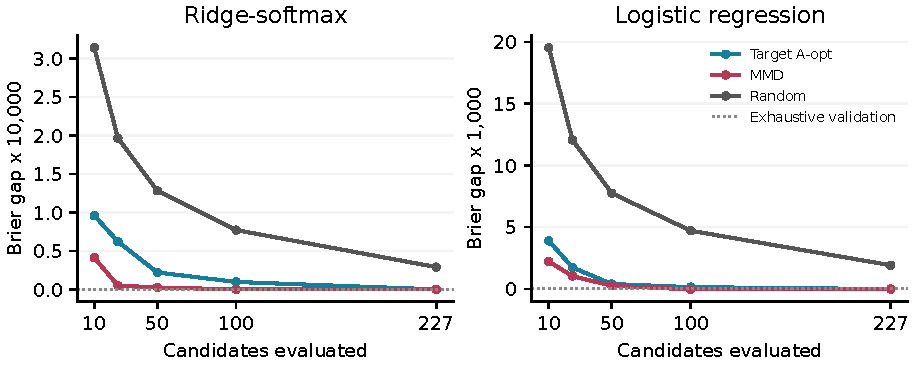
\includegraphics[width=\linewidth]{decision_budget.pdf}
\caption{Mean final test Brier minus the exhaustive-validation choice is plotted against the number of candidates evaluated. The two panels use different vertical scales. The zero line is a validation-selected model, not the test oracle. Curves are post-hoc summaries of the four archived projection seeds; the horizontal axis counts fits, not measured runtime.}
\label{fig:budget}
\end{figure}
\label{app:budget}
The post-hoc budget audit uses the four new projection seeds and both readouts without selecting a favorable seed. For each task and endpoint, exhaustive validation chooses its combination using validation losses only. Its test loss is then the paired reference for the frozen shortlist choices. In contrast, the empirical test oracle remains a lower audit reference. All five original budgets are retained.

\begin{table}[ht]
\centering
\caption{Final logistic-regression Brier and the rate of exceeding the exhaustive-validation reference by more than $0.005$ are reported. Means average random repetitions before encoders and seeds within each domain, then the six domains. The tolerance is exploratory, not a new success gate.}
\label{app:budget-table}
\begin{tabular}{lrrr}
\toprule
Screen & Fits & Test Brier & Gap $>0.005$ (\%)\\
\midrule
Random & 227 & 0.866030 & 15.52 \\
Target A-opt & 50 & 0.864511 & 2.08 \\
MMD & 50 & 0.864365 & 2.08 \\
Exhaustive validation & 455 & 0.864118 & 0.00 \\
\bottomrule
\end{tabular}

\end{table}

We report absolute-gap sensitivity grids of $0.001,0.005,0.01$ for Brier, $0.01,0.05,0.1$ for NLL, and $0.5,1,2$ percentage points for error. Exceedance indicators are computed before averaging random repetitions; thresholding an averaged loss would answer a different question. Descriptive paired bootstrap ranges use 2,000 resamples of the six domain averages. They do not account for dependence induced by shared source pools, validation resampling, or independent datasets. All endpoint curves, paired domain differences, and threshold rates are in \path{results/target_conditioned/revision_20260922/budget_audit/}. The script \path{scripts/analyze_e2b_decision_budget.py} verifies recorded loss hashes and constructs the exhaustive reference from validation files.

\begin{figure}[t]
\centering
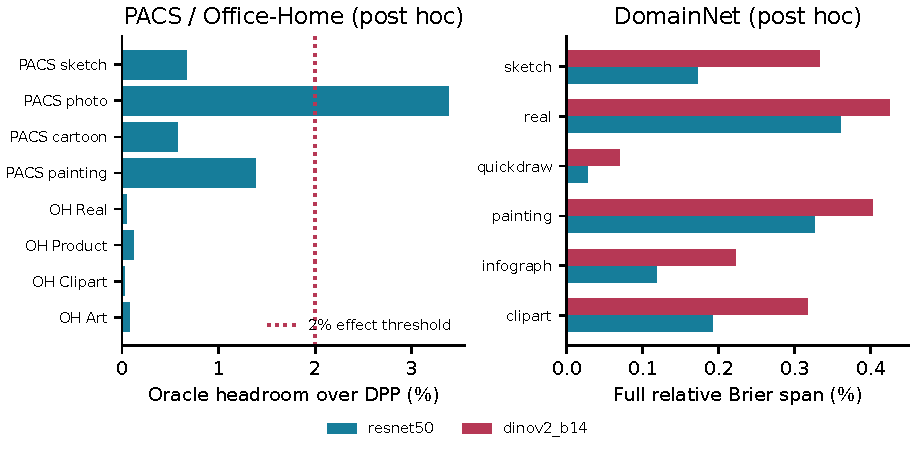
\includegraphics[width=\linewidth]{headroom_diagnostics.pdf}
\caption{The panels report post-hoc diagnostics for different candidate families. The left panel shows oracle Brier improvement over DPP, averaging encoders within each PACS/Office-Home target. The right panel shows relative best-to-worst Brier spans for the original DomainNet tasks. The original evaluation thresholds are unchanged.}
\label{fig:diagnostics}
\end{figure}

\subsection{Loss resolution and test-sample stability}
The post-hoc loss-span diagnostic in Appendix Figure~\ref{fig:diagnostics} puts the original regret criterion in context. Every candidate's relative Brier regret lies below the $5\%$ threshold, so that threshold cannot distinguish successful screens in this experiment. Recall provides the more informative comparison, but it raises another question: how sensitive is the test top ten to the sampled test examples?



A CUDA reconstruction first reproduces all original Brier top-ten sets. We then apply paired test-example bootstrap resampling while fixing fitted models and validation choices. Although resampled and original top-ten sets overlap by only $\BootstrapOverlap\%$ on average, Target A-opt and MMD retain $\BootstrapRecall\%$ and $\BootstrapMMDRecall\%$ of the resampled top tens. Broad shortlists are less sensitive than exact rank membership to these test-sample changes.

Changing the metric has a larger effect on which combinations count as good: the original Brier and classification-error top tens overlap by only $\BrierErrorOverlap\%$ on average. A screen should therefore be evaluated against the intended deployment metric, even when its average recall is high for several metrics. The resampling protocol and additional metric comparisons appear in the main paper protocol appendix.

\subsection{Candidate construction and domain controls}
\label{app:construction}
The fixed challenge uses projection seed $20260917$, both encoders, and both readouts. Each domain's original 1,536 source images are sorted by SHA-256 of a fixed seed, domain identifier, and sample identifier, then partitioned into three blocks of 512. No labels, feature values, or outcomes determine membership. Target-selection, validation, and test sets do not change. The original construction is rerun as a control: all 65,520 recorded validation/test loss values agree exactly with the corresponding earlier seed. Repartitioning does not reuse CLIP stratum labels, but still conditions on the originally selected source images; it is neither an independent dataset nor a new test sample.

Mean matching minimizes $\|\bar h_S-\bar h_T\|_2^2$, the linear-kernel MMD score. Domain matching additionally uses source-domain identifiers: it replaces each block moment by its full source-domain moment, weights these moments by the candidate's domain sample proportions, and minimizes squared Frobenius distance to the target moment. The original challenge breaks ties lexicographically. Because domain matching creates many structural ties, an additional post-hoc audit randomizes the order within each tied domain-composition stratum using 20 fixed seeds. It freezes every new validation choice before reading test losses and does not refit or change classifier parameters. The original tie protocol remains available in the released curves.

\begin{table}[ht]
\centering
\caption{The construction challenge uses logistic Brier. Final loss is validation-selected at $s=50$. The last columns measure retention of one empirical optimum when half of each non-singleton domain-composition stratum is kept, not final selection accuracy. Means average strata and encoders within targets, then six targets. Domain matching uses 20 randomized tie orders for final loss; its within-stratum entry is the exact uniform-tie expectation.}
\label{app:construction-table}
\begin{tabular}{lrrrr}
\toprule
 & \multicolumn{2}{c}{Final Brier ($s=50$)} & \multicolumn{2}{c}{Within-composition (\%)}\\
Screen & Original & Hash & Original & Hash\\
\midrule
Target A-opt & 0.863170 & 0.869699 & 77.22 & 55.83 \\
MMD & 0.863110 & 0.869257 & 76.11 & 55.00 \\
Mean matching & 0.863713 & 0.873038 & 75.28 & 57.78 \\
Domain moment (random ties) & 0.863667 & 0.869356 & 45.68 & 45.68 \\
Random & 0.870013 & 0.874244 & 45.04 & 45.31 \\
\bottomrule
\end{tabular}

\end{table}

There are 20 strata of nine candidates and ten of 27 per target; five singleton strata are excluded. Within a stratum, every candidate uses the same domain multiplicities and total sample count. Random repeats are averaged first, followed by strata, encoders, and target domains. A domain-only score is constant inside a stratum, giving expected optimum retention $(20\cdot4/9+10\cdot13/27)/30=45.68\%$ under uniform ties. Lexicographic within-stratum results are recorded but not interpreted as domain discrimination.

After hash repartitioning, logistic classification-error optimum retention is $41.94\%$ for Target A-opt and $35.28\%$ for MMD, versus $45.75\%$ for random selection. Mean Brier omission remains lower than random for both scores, but the advantage is smaller than on the original blocks. These metric-dependent observations describe conditional ranking performance; they do not establish a population guarantee or isolate the causal contribution of heterogeneity from the properties of this particular partition.

The complete curves and domain-conditional audits are in \path{results/target_conditioned/revision_20260922/challenge_summary/}; randomized domain ties are in \path{results/target_conditioned/revision_20260922/domain_tie_audit/}. The raw three-stage records bind candidate membership, source features, configuration, upstream choices, and numerical payloads by hashes. Local summaries verify all numerical hashes and upstream seals; frozen model hashes were checked on the server before test access.

\subsection{Matched quality and computation costs}
\label{app:cost}
The timing study uses the original candidate construction and projection seed $20260917$. Each encoder--target--readout task runs Target A-opt, MMD, random screening, and exhaustive validation independently, with three repetitions and a seeded method order. BLAS uses one thread. Shortlist checkpoints measure cumulative elapsed time after a single ranking; no fitted model is shared across methods. Ridge lazily caches each used block's float64 Gram and label right-hand side, including in exhaustive search. Preliminary float32-Gram ridge timings are retained in the archive but excluded from all tables.

Every timed validation loss and choice is checked against the frozen scientific audit. Quality in Figure~\ref{fig:cost} uses the actual choices from these same three runs, with Brier, NLL, and error each using its matching validation metric. Thus the random quality coordinates here average three timed rankings, not the 20 rankings in the main scientific audit. We first average repetitions within each task, then encoders within targets and the six targets equally; timing medians are retained as diagnostics.


\begin{figure}[t]
\centering
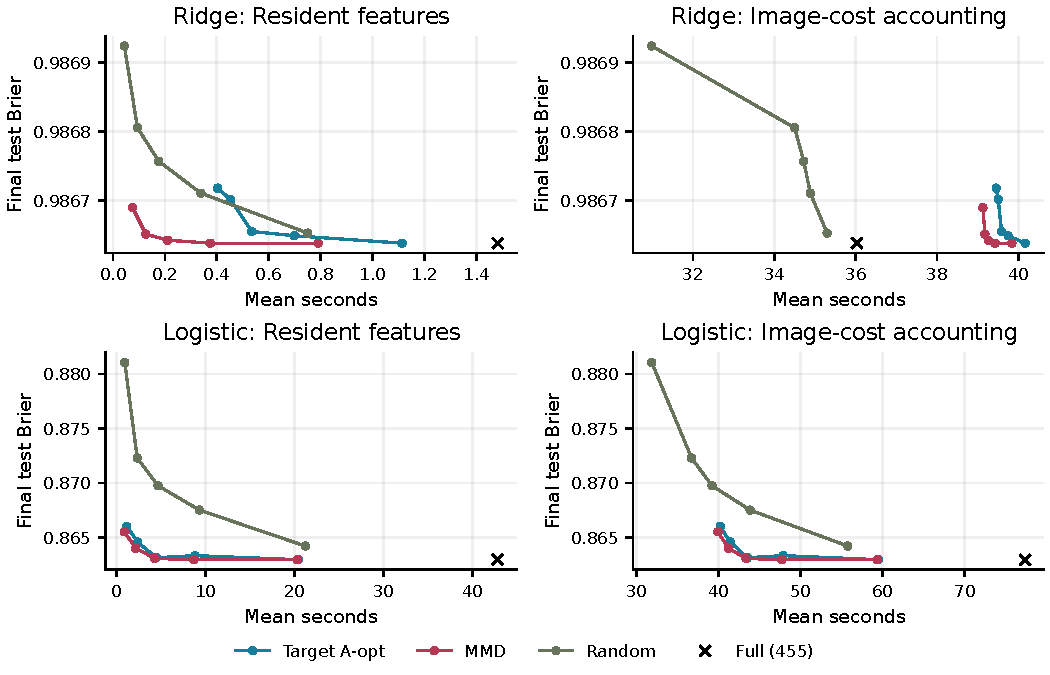
\includegraphics[width=\linewidth]{quality_cost.pdf}
\caption{Final test Brier is plotted against matched decision time and additive image-cost accounting. Each curve has budgets $10,25,50,100,227$; crosses mark exhaustive validation over 455 candidates. Rows have different vertical scales. Means use two encoders, six targets, and three independent executions per method. Raw-image costs exclude pool construction, downloads, cache serialization, and test auditing.}
\label{fig:cost}
\end{figure}

The resident scope excludes loading stage bundles, checking their integrity, and projecting cached features. Table~\ref{app:cache-table} accounts for these operations separately for two six-target encoder batches. Target-aware methods load both selection and validation bundles; random and exhaustive methods need only validation bundles. Shared preparation is charged once per encoder batch, not converted into a fictitious single-task time.

\begin{table}[ht]
\centering
\caption{Disk-cache batch costs in seconds include input loading, integrity checks, projection, and all twelve encoder--target decisions. They are totals for two six-target batches, whereas the main paper cost table reports per-task means. The choices and losses do not change.}
\label{app:cache-table}
\begin{tabular}{lrrrr}
\toprule
Readout & Target A-opt (50) & MMD (50) & Random (227) & Full (455)\\
\midrule
Ridge & 9.35 & 5.46 & 10.40 & 19.18\\
Logistic & 56.77 & 54.63 & 255.89 & 515.12\\
\bottomrule
\end{tabular}

\end{table}

Raw-image profiling measures model initialization, image reads and hash checks, decoding, preprocessing, inference, CPU feature transfer, and normalization/projection. Each source block is timed separately; random screening is charged only for the union of blocks in its actual prefix, while geometric scoring and exhaustive validation use all 15 eligible source blocks. Each method also needs target-validation features; only target-aware scores need the target-selection sample. No test images are processed. The fixed candidate inventory is supplied to this measurement, so CLIP-based pool construction is outside its scope.

The machine uses an Intel Xeon Platinum 8352V CPU and an NVIDIA vGPU-32GB. Feature extraction uses CUDA 12.4, PyTorch 2.5.1, float32 inference without TF32, batch size 64, and four data-loading workers. The readout stack uses NumPy 1.26.4, SciPy 1.16.1, and scikit-learn 1.7.1. Feature components are measured in one pass, with operating-system disk caches left unchanged. Block-level loader startup is included. The totals therefore describe this measured implementation and reuse scenario, not a hardware-independent speedup.

All 32 quality/time curve entries, three loss endpoints, paired differences, and 384 task-level budget entries are in \path{results/target_conditioned/revision_20260922/cost_summary/}. Standalone timing runs and per-block feature profiles accompany them. The manuscript verifier independently reconstructs the matched quality coordinates, random block unions, and all additive totals from those records.

\section{Connections to Recent Data-Selection Methods}
\label{app:related-selection}
Recent selection methods differ in what they select, which representation describes relevance, and what information selection can access. These distinctions locate the present framework and determine how a future comparison should be constructed. The methods discussed here provide literature context; our measured comparators remain those in the main paper protocol.

Transductive active learning separates an accessible sampling region from a prediction target region \citep{hubotter2024transductive}. ITL reduces target entropy, whereas VTL reduces the sum of target predictive variances. Their Gaussian-process formulation explains how an observation can be useful for a target without being drawn from that target region. The variance objective is the closest connection to the shared-model risk identity in the paper: source geometry matters through the uncertainty remaining at target covariates. We evaluate complete, fixed pool combinations and then validate retained predictors, rather than sequentially acquiring individual observations.

SIFT makes redundancy important to target-specific selection \citep{hubotter2025sift}. It selects fine-tuning sequences by the uncertainty remaining about a prompt after conditioning on previously selected sequences. Consequently, an example's relevance depends on what has already been selected, not just its distance to the prompt. This provides a useful perspective on pooled Gram matrices, whose combined coverage also depends on cross-pool alignment. SIFT's experiments concern prompt-specific language-model fine-tuning; here the encoder remains frozen and the supervised stage compares readouts trained on different pool unions.

SkMM addresses the bias--variance tradeoff of selecting data for high-dimensional fine-tuning \citep{dong2024skmm}. Gradient sketching first identifies a low-dimensional parameter subspace with controlled approximation bias; moment matching then controls variance within that subspace. Its gradient representation comes from model derivatives, so it should not be conflated with label-dependent loss-gradient selection. SkMM matches selected data to the original dataset, whereas our target moment is estimated from a separate target-selection sample. Both use matrix geometry, but our fixed feature projection does not perform SkMM's gradient-space construction.

TSDS balances distribution alignment and diversity by optimizing sampling probabilities with an optimal-transport objective \citep{liu2024tsds}. Its density-aware regularizer reduces concentration on near-duplicate candidates, and its metric space can use semantic embeddings or model-specific representations. TAROT builds transport costs from projected, whitened, normalized loss-gradient features \citep{feng2025tarot}. Whitening reduces the dominance of correlated gradient directions before matching the selected and target distributions. Unlike our unlabeled screen, its supervised loss-gradient construction includes both inputs and labels. These are relevant transport-based comparison methods, but their sample-level outputs must be reconciled with our fixed-block candidate family. A frozen-embedding OT score would be a useful controlled adaptation, not a reproduction of TAROT's loss-gradient method.

The covariance-matching analysis of \citet{rezaei2026synthetic} studies a predictor trained on real data augmented with synthetic data under high-dimensional linear regression. It characterizes test error and establishes covariance-matching optimality under specified conditions. This gives matching a risk-based motivation beyond simple geometric resemblance. The distinction between centered covariance and uncentered second moments matters here: the second-moment MMD criterion in the paper compares the latter on frozen features. Our classification shortlists address a different training and selection setting from the synthetic-augmentation analysis.

A comparison with these methods would need to hold the candidate family, sample cost, target-data roles, and final validation rule fixed. Extra label access would require a separately identified information setting. Feature or gradient construction, transport optimization, screening, and supervised evaluation would all enter the cost account. This follows the selection-plus-training budget principle of \citet{yin2025} and makes the comparison about the final predictor obtained for the available computation, rather than the screening score alone.

\section{Archived pool-query and calibration results}

The extension uses all four additional archived projection seeds, the same candidate memberships, and seed-specific rankings and validation/test losses. The fixed A-opt and MMD comparators take their archived prefixes, and the random comparator averages 20 archived orders per seed, encoder and target. Every policy observes only its queried validation scores. We lock all traces before opening test scores, and the full reference minimizes validation loss across all 455 candidates. The six-domain means weight encoders equally within each domain and then weight domains equally. An exceedance is a signed Brier gap strictly above $0.005$, computed separately for each seed and domain. Across the 48 seed--encoder--domain units, pool only at 25 recovers 45 full-validation winners, and MMD at 50 recovers 42. The archive was used for earlier analyses. Projection and readout variation on the shared data supports a within-benchmark sensitivity check. This replay reuses fitted models' validation and test scores. Appendix~\ref{app:server-timing} measures elapsed time in separate runs with fresh fits at the original projection seed.

\begin{table}[ht]
\centering
\caption{Archived DomainNet logistic test Brier, averaged over six domains and two encoders per seed. The gap is pool only at 25 queries minus fixed MMD at 50. Full search selects by validation over 455 candidates.}
\label{tab:pool-query}
\begin{tabular}{lrrrr}
\toprule
Projection seed & Pool only (25) & Fixed MMD (50) & Full (455) & Gap to MMD \\
\midrule
20260917 & 0.863052 & 0.863110 & 0.862992 & $-0.000058$ \\
20260918 & 0.865693 & 0.866049 & 0.865646 & $-0.000356$ \\
20260919 & 0.864673 & 0.864555 & 0.864555 & $+0.000118$ \\
20260920 & 0.863278 & 0.863748 & 0.863278 & $-0.000470$ \\
\midrule
Mean & 0.864174 & 0.864365 & 0.864118 & $-0.000191$ \\
\bottomrule
\end{tabular}
\end{table}

\subsection{Other screening checks}
In a matched DomainNet logistic comparison at 50 fits, Target A-opt gives mean test Brier $0.864104$, versus $0.896467$ for linear target energy, which uses the same moments without inverse weighting. At 227 fits, Target A-opt and MMD both give $0.863757$, versus $0.873177$ for linear target energy. A validation-only stopping rule calibrated on the other five domains saves 2.08 queries on average for MMD relative to fixed 50 and increases queries for Target A-opt. These retrospective checks share source pools across domains. On Office-Home at 50 fits, Target A-opt improves on target energy by $0.030215$ in mean Brier, and MMD is slightly better than Target A-opt. On BloodMNIST, with constructed pools and an internal holdout, all differences against Target A-opt fall below the prespecified $0.005$ threshold.

\section{Server timings with resident features}
\label{app:server-timing}
Both timing studies use six DomainNet target domains, two encoders, and the original projection seed 20260911. They start with projected features in memory and end when validation selects a winner. Feature extraction and test evaluation fall outside the timed interval.

\paragraph{Logistic regression.}
We independently fit each candidate in three runs per policy and thread setting, rotating the policy order. Timing includes candidate preparation, screening or query selection, fitting, and validation. The four-thread setting dispatches independent fits on four threads, with one native library thread per fit and worker initialization outside the timed interval. Both pool policies can fit the first 15 candidates in parallel. Sequential 25 uses each new validation score before choosing the next candidate. Two-batch 25 ranks the remaining candidates once using the first 15 scores and dispatches the next ten together. MMD ranks candidates from the resident features and can dispatch all 50 fits together.

\begin{table}[ht]
\centering
\caption{Logistic selection time in seconds. We take the median across three repeats within each encoder--domain unit, then the median across the 12 units. Test Brier weights the units equally.}
\label{tab:pool-server-timing}
\begin{tabular}{lrrrr}
\toprule
Policy & Fits & One thread & Four threads & Test Brier \\
\midrule
Sequential & 25 & 1.384 & 0.793 & 0.863951 \\
Two-batch & 25 & 1.390 & 0.453 & 0.863951 \\
MMD & 50 & 2.666 & 0.824 & 0.863951 \\
Full validation & 455 & 25.702 & 7.554 & 0.863757 \\
\bottomrule
\end{tabular}
\end{table}

All 288 runs match the archived query order and winner. The median paired speedups over MMD 50 for sequential and two-batch 25 are $1.92\times$ and $1.91\times$ at one thread, and $1.04\times$ and $1.86\times$ at four. The two pool policies select the same winners on this projection. Their mean Brier gaps are $+4.26\times10^{-7}$ to MMD 50 and $+0.000194$ to full validation, with no encoder--domain gap above $+0.005$ against either reference. Replaying two-batch versus sequential at 25 on the four additional projections gives a mean gap of $+0.000254$, with one of 48 encoder--seed--domain units above $+0.005$.

\paragraph{Calibrated ridge regression.}
From resident features and precomputed rankings, we time block statistics, fitting ridge with $\lambda=1$, validation logits, the temperature grid on one validation half, and selection on the other half. The 360 timed runs across calibrated and uncalibrated settings reproduce the archived outcomes. The table averages the three-run medians across 12 units. Temperature search accounts for about $93$--$94\%$ of calibrated time. These timings condition on the shortlist rankings being available. The image-cost comparison in the main paper cost section uses the original uncalibrated ridge protocol.

\begin{table}[ht]
\centering
\caption{Ridge selection time in seconds from resident features and precomputed rankings. Test Brier is for reselection after temperature calibration.}
\label{tab:ridge-server-timing}
\begin{tabular}{lrrrr}
\toprule
Policy & Fits & Uncalibrated & Calibrated & Test Brier \\
\midrule
Target A-opt & 50 & 0.070 & 1.114 & 0.725347 \\
MMD & 50 & 0.071 & 1.114 & 0.727958 \\
Target A-opt & 227 & 0.300 & 5.009 & 0.725498 \\
MMD & 227 & 0.296 & 5.064 & 0.725498 \\
Full validation & 455 & 0.586 & 10.047 & 0.725498 \\
\bottomrule
\end{tabular}
\end{table}

\section{Further analysis of the new experiments}

\subsection{Diagnosing the additive approximation}
For Optdigits, we compare the predictions after 15 and 25 queries on the same set of candidates still unqueried after query 25. Averaged across four hash-partition seeds, prediction $R^2$ rises from $0.581$ to $0.637$ and top-25 validation recall rises from $0.47$ to $0.61$. For PC1, prediction $R^2$ rises from $-21.45$ to $-7.57$ and recall from $0.01$ to $0.02$. A retrospective fit to all 455 validation scores reaches $R^2$ of $0.851$ for hash and $0.169$ for PC1. In a post-hoc five-fold diagnostic, adding pool-pair features raises predictive $R^2$ from $0.840$ to $0.995$ for hash and from $0.095$ to $0.910$ for PC1. Each fold uses 364 candidate losses for fitting. The results suggest that interactions can explain a substantial part of PC1's approximation error. These diagnostics access losses unavailable to the 25-fit selector. A check at deployment would need additional held-out candidate queries charged to the budget, since 15 independent rows can interpolate their 15 observed scores.

\subsection{Additional best-arm diagnostics}

We evaluate three ways to return the final model. With \emph{observed} termination, the policy uses its whole budget $B$ and returns the queried candidate with the lowest observed validation loss. With \emph{recommend} termination, it uses $B-1$ policy queries and trains the best predicted unused candidate with the remaining fit, then returns the observed validation winner among all $B$. With \emph{native prediction}, it returns the predicted best candidate after $B-1$ policy queries. It uses the last fit on that prediction if unseen, or on the best predicted unseen candidate otherwise. We lock selections before the new test audit. Tables use recommend termination for the linear-design baselines so a predicted winner can be trained within the same budget used by the other methods. On DomainNet/PC1, giving D-design this final fit reduces its mean test Brier gap to the full-validation reference from about $0.0128$ to $0.0010$. Validation simple regret, the selected candidate's validation loss minus the minimum over all candidates, measures the selection objective directly. Sequential 25 has mean regret $0.000085$ on the 48 DomainNet configurations, with $0.000949$ for D-design, $0.001600$ for XY-design, $0.000768$ for the scale-matched LinGapE adaptation and $0.004644$ for MMD 25. On Optdigits/PC1, XY-design reduces regret from $0.059715$ for sequential 25 to $0.009403$. At 100 fits, sequential, D-design and XY-design give test Brier of $0.391922$, $0.341057$ and $0.341944$ respectively in this failure setting.

\subsubsection{Original OD-LinBAI at a feasible budget}
The phase allocation in \citet[Eq.~1]{yangtan2022linbai} has no positive stage budget at $B=25$ for 455 arms of dimension 15. We run the published allocation with nominal budget 200, using phase multiplier 16.5 and survivor counts 8, 4, 2 and 1. The first G-optimal design is uniform on a 35-triple Steiner system, giving the same incidence information matrix as the uniform design on all triples. Later phases solve the design within the current incidence span, and each phase estimates losses from that phase's scores. This uses 91--97 pulls and 41--43 distinct model fits. On DomainNet the native recommendation recovers the full-validation winner in 20/24 hash and 22/24 PC1 configurations. At matched distinct-fit counts the native rule and sequential give Brier $0.922337$ versus $0.922212$ on DomainNet/hash, and $0.909925$ versus $0.909978$ on DomainNet/PC1. On Optdigits/PC1, native prediction gives $0.440156$, the observed-winner fallback gives $0.371922$, and sequential gives $0.402315$ at the same 43 distinct fits. Memoizing repeated deterministic scores preserves the actual count of trained models. The stochastic analysis assumes new observations from repeated pulls.

We separately rerun the fit-and-select procedure from in-memory features, including ranking or query computation, model fitting and validation. Test scoring, cache decoding and integrity checking are outside the timed decision. Tables aggregate the six DomainNet targets using hash pools and the first seed, with three rotated repeats per strategy. Optdigits uses its first hash seed and three repeats. Each fitting worker uses one BLAS thread. We use a shared Intel Xeon Gold 6133 server, with our other campaign compute paused. In the separate linear-design timing, the median over 18 DomainNet one-worker runs is $3.309$ s for sequential 25, $3.352$ s for D-design, $3.338$ s for A-design, $3.349$ s for G-design and $3.356$ s for the $0.001$ LinGapE adaptation. The exact greedy XY implementation takes $8.434$ s, including $5.126$ s for selection computation. That implementation searches all candidate pairs for each proposed query.

We check the first DomainNet hash seed at five nested projection dimensions. Each candidate uses the first validation half to fit temperature over 81 log-spaced points from $0.01$ to $100$, or jointly choose $\lambda\in\{0.1,1,10\}$ and temperature. All three arms, including the uncalibrated $\lambda=1$ reference, use the other validation half for choosing the winning candidate. Geometric rankings retain their original definitions. Tuning $\lambda$ incurs three supervised fits per candidate, so 25 candidate queries cost 75 fits. the main paper ridge sensitivity table reports calibration and selection with matched settings within each column. Higher dimensions improve the full-validation score in this study, and some dimensions and regularization settings increase the gap of the 25-query selection. For Optdigits/PC1, tuning reduces sequential Brier from $0.262615$ to $0.246578$, with calibrated full validation at $0.170425$ in both arms. The fresh ridge runs share candidate fitting and calibration work across policies for the quality audit. Appendix~\ref{app:server-timing} provides independent time measurements for the original fixed-dimension, fixed-$\lambda$ ridge study.

\subsection{Exploratory scale and budget checks}
A constructed Clipart inventory uses 128-dimensional ResNet-50 features and 768 rows per candidate. Across inventories of 455, 1,140, 2,300 and 4,060 candidates, an exact bound-based screen reproduces the exhaustive Cholesky Target A-opt shortlists. At 4,060 candidates, the top-50 ranking time is $1.23$ s versus $2.35$ s for exhaustive scoring (three-run medians). This tests static ranking cost. The pool-query quality experiments use the 455-candidate family.

A separate leave-one-target-domain archive replay calibrates a validation-based stopping rule on the other domains. For fixed MMD ranking it evaluates $47.92$ candidates on average versus 50 for the fixed budget, saving $2.08$ queries. Both settings have zero of six domain-average test Brier gaps above $+0.005$ to full validation. The same protocol uses more fits than the fixed budget for Target A-opt and random ranking. This single-projection comparison is retrospective and shares source pools across targets. It leaves prospective budget selection open.

\bibliography{references}
\bibliographystyle{iclr2027-style/iclr2027_conference}
\end{document}
